\documentclass[10pt,a4paper]{amsart}
\usepackage[margin=19mm]{geometry}
\usepackage{amsmath,amssymb,mathtools}
\usepackage[scr=rsfs,cal=euler]{mathalfa}
\usepackage{xfrac}
\usepackage[unicode,hidelinks,bookmarks=false]{hyperref}
\newcommand{\ie}{i.e.\ }
\newcommand{\cf}{cf.\ }
\newcommand{\resp}{respectively\ }
\newcommand{\Subsection}{\subsection}
\providecommand{\nobreakdash}{\nobreak\hbox{-}}
\setlength{\emergencystretch}{2em}
\multlinegap0pt
\usepackage{tikz}
\usepackage{mathtools}
\usepackage{amssymb}
\usepackage[shortlabels]{enumitem}
\usepackage{xcolor}
\usepackage{tcolorbox}
\newtheorem{proposition}{Proposition}
\newcommand{\interior}[1]{\mathrm{int} \, #1}
\newcommand{\realNumbers}{\mathbb{R}}
\title{On quantum channels: extreme points, topology, and categorical properties}
\author{J. M. S. T. da Silva}
\date{Source: arXiv:2608.20689v1 (CC BY 4.0)}
\begin{document}
\maketitle

\noindent\emph{Source and licence.} On quantum channels: extreme points, topology, and categorical properties. Version arXiv:2608.20689v1 (CC BY 4.0), distributed by arXiv under the Creative Commons Attribution 4.0 International licence, http://creativecommons.org/licenses/by/4.0/, as recorded in the arXiv licence metadata for this exact version and shown on the abstract page https://arxiv.org/abs/2608.20689v1. Full licence notice: \texttt{licenses/arxiv-2608.20689-CC-BY-4.0.txt}.\par\smallskip

\noindent\textit{Editorial scope.} Counted unit: the article's proposition proposition (source0.tex lines 15020--15022). The article's complete original proof of it is delivered with it (source0.tex lines 15023--15557, one \texttt{proof} environment of 535 lines). No mathematics is written, repaired or re-derived: the statement and the proof are the article's own lines, in the article's own notation, and no retained line is substituted or re-flowed.  No further source-local context is needed: every cross-reference of every retained line resolves inside the two delivered spans.  Nothing was omitted from any retained span, so the package carries no omission record.  No retained line contains a citation, so the wrapper carries no bibliography and no bibliography entry.  The retained lines contain the article's own diagram code, which the wrapper typesets with the standard tikz packages; no image file is delivered and the package declares no asset dependency.  Editorial formatting only, in addition: an AMS \texttt{amsart} preamble that restates the article's own declarations and macros used by the retained lines, namely the environments \texttt{proposition} on separate counters, together with the standard packages those lines need.  The retained environments print in this document as Proposition 1 in order of appearance, whereas the article prints the same items with the numbering of its own full document.  The complete native source of the article as distributed in the arXiv e-print for this exact version is bundled unchanged as \texttt{sources/208200/source0.tex}.
\begin{proposition}{}{compact convex set with non empty interior}
	Let $C \subseteq \realNumbers^n$ be a compact convex subset with $\interior{C} \neq \varnothing$. Then $C$ is homeomorphic to the closed unit ball $\overline{B(0,1)} \subseteq \realNumbers^n$.
\end{proposition}

\begin{proof}
	Let $z \in \interior C$ and define $C' \coloneqq C-z = \{x-z \mid x \in C\}$. Then $C'$ is a compact convex set homeomorphic to $C$, with $0 \in \interior C'$. The idea is to pick a line segment of $C'$ which starts at 0 and ends at the furthest point along some direction which is still inside $C'$, and then rescale such line segment so that its length becomes 1. First we define a function $R$ that gives the length $R(x)$ of the line segment determined by the direction of a unit vector $x \in S^{n-1}$, where
	\begin{equation}
		S^{n-1} = \{x \in \realNumbers^n \mid ||x|| = 1 \}
	\end{equation}
	is the unit sphere. Since $0 \in \interior C'$, there exists some $r_{min} > 0$ such that
	\begin{equation}
		\label{equation: smaller ball}
		\overline{B(0,r_{min})} \subseteq C'.
	\end{equation}
	$C'$ is also compact, so it is bounded, which implies that there is some $r_{max} \geq r_{min}$ such that
	\begin{equation}
		\label{equation: bigger ball}
		C' \subseteq \overline{B(0,r_{max})}.
	\end{equation}
	For this reason, we must have that
	\begin{equation}
		r_{min} \leq R(x) \leq r_{max}.
	\end{equation}
	The function $R$ is then defined as follows:
	\begin{align*}
		R \colon S^{n-1} &\longrightarrow [r_{min}, r_{max}] \\
		x &\longmapsto \max \left\{\lambda > 0 \mid \lambda x \in C' \right\}.
	\end{align*}
	We must prove that this definition is correct, that is, that the maximum exists and that it is in the interval $[r_{min}, r_{max}]$. For the existence, first notice that
	\begin{equation}
		r_{min} \in \{\lambda > 0 \mid \lambda x \in C' \},
	\end{equation}
	because of equation \ref{equation: smaller ball}. Equation \ref{equation: bigger ball} implies that
	\begin{equation}
		\{\lambda > 0 \mid \lambda x \in C' \} \subseteq (0,r_{max}].
	\end{equation}
	This shows that
	\begin{equation*}
		\{\lambda > 0 \mid \lambda x \in C' \}
	\end{equation*}
	is a non empty and bounded set, therefore it has a supremum. The supremum is a maximum iff it is in the set
	\begin{equation*}
		\{\lambda > 0 \mid \lambda x \in C' \}.
	\end{equation*}
	Let
	\begin{equation}
		s \coloneqq \sup \{\lambda > 0 \mid \lambda x \in C' \}.
	\end{equation}
	From the definition of supremum, there is an increasing sequence in the set that converges to it. That is, there is an increasing sequence $(\lambda_m)_{m \geq 1}$, with
	\begin{equation}
		\lambda_m > 0,
	\end{equation}
	\begin{equation}
		\lambda_m x \in C',
	\end{equation}
	such that
	\begin{equation}
		\lim_{m \to \infty} \lambda_m = s.
	\end{equation}
	Since $C'$ is compact, it is also closed. This implies that
	\begin{equation}
		\lim_{m \to \infty} \lambda_m x \in C',
	\end{equation}
	so
	\begin{equation}
		s x \in C'.
	\end{equation}
	Also, since the sequence $(\lambda_m)_{m \geq 1}$ is increasing and $\lambda_m > 0$, it follows that
	\begin{equation}
		s \geq \lambda_1 > 0.
	\end{equation}
	This proves that the supremum is in the set:
	\begin{equation}
		s \in \{\lambda > 0 \mid \lambda x \in C' \}.
	\end{equation}
	Therefore, the maximum from the definition of $R$ exists. Since the set
	\begin{equation*}
		\{\lambda > 0 \mid \lambda x \in C' \}
	\end{equation*}
	contains $r_{min}$ and is bounded from above by $r_{max}$, it follows that
	\begin{equation}
		\label{equation: R bounds}
		R(x) \in [r_{min}, r_{max}].
	\end{equation}
	This concludes that the definition of $R$ is correct.
	
	Having defined the function $R$, we can use it to rescale the line segments. The function that does the rescaling is defined as follows:
	\begin{align*}
		\varphi \colon C' &\longrightarrow \overline{B(0,1)}\\
		x &\longmapsto \begin{cases}
			\frac{x}{R(x/||x||)} &\text{ if } x \in C' \setminus \{0\}\\
			0 &\text{ if } x=0.
		\end{cases}
	\end{align*}
	To finish the proof, we need to prove that $\varphi$ is a homeomorphism. First we'll prove that $R$ is continuous.
	
	Let $x, x' \in S^{n-1}$. Taking them to be close enough, they must satisfy that
	\begin{equation}
		\label{equation: x x' > 0}
		x \cdot x' > 0.
	\end{equation}
	For instance, this is the case if we assume that
	\begin{equation}
		\label{equation: x-x' close enough}
		||x-x'|| \leq ||x|| = 1.
	\end{equation}
	With such assumption, we have that
	\begin{align*}
		x \cdot x' &\stackrel{(i)}{=} \frac{||x||^2 +||x'||^2 -||x-x'||^2}{2} \\
		&\stackrel{(ii)}{\geq} \frac{||x'||^2}{2} \\
		&\stackrel{(iii)}{>} 0.
	\end{align*}
	In $(i)$ was used that $||y||^2 = y \cdot y$, to find and expression of the scalar product in terms of the norm; in $(ii)$ was used equation \ref{equation: x-x' close enough}; in $(iii)$ was used that $x' \neq 0$. With this result, the vectors $x$ and $x'$ are in the same half of the unit sphere $S^{n-1}$.
	
	Next we find a lower bound for $R(x')$ from the information about $x$ and $C'$. By symmetry, this will also give a lower bound for $R(x)$. Combining both bounds we'll get that $R$ is continuous. First rescale $x$ and $x'$ to the maximum norm possible, but remaining inside $C'$. We get the following vectors:
	\begin{equation}
		\widetilde{x} \coloneqq R(x) x,
	\end{equation}
	\begin{equation}
		\widetilde{x'} \coloneqq R(x') x'.
	\end{equation}
	We have a special case when $R(x) = r_{min}$. To avoid separating into multiple cases, we'll work with a strictly smaller radius. Let $r_s \in \realNumbers$ be any such that
	\begin{equation}
		0 < r_s < r_{min}.
	\end{equation}
	In this way,
	\begin{equation}
		R(x) > r_s
	\end{equation}
	for any $x \in S^{n-1}$. Since $x, x' \in S^{n-1}$, these vectors are linearly dependent iff $x' = \pm x$. For computing $\lim_{x' \to x} R(x')$ we can assume that $x' \neq x$. We are assuming that $x \cdot x' > 0$, as in equation \ref{equation: x x' > 0}, so $x' \neq -x$. This implies that $(x,x')$ is linearly independent. Consider the following picture:
	\begin{center}
		\tikzset{every picture/.style={line width=0.75pt}} %set default line width to 0.75pt        
		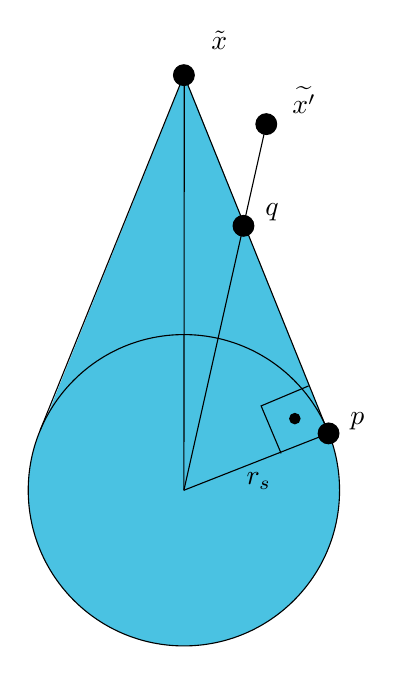
\begin{tikzpicture}[x=0.75pt,y=0.75pt,yscale=-1,xscale=1]
			%uncomment if require: \path (0,306); %set diagram left start at 0, and has height of 306
			
			%Shape: Triangle [id:dp13002420225256628] 
			\draw  [draw opacity=0][fill={rgb, 255:red, 74; green, 194; blue, 226 }  ,fill opacity=1 ] (175.2,25) -- (244.7,197.6) -- (105.7,197.6) -- cycle ;
			%Shape: Circle [id:dp8478434896942522] 
			\draw  [fill={rgb, 255:red, 74; green, 194; blue, 226 }  ,fill opacity=1 ] (100,225) .. controls (100,183.58) and (133.58,150) .. (175,150) .. controls (216.42,150) and (250,183.58) .. (250,225) .. controls (250,266.42) and (216.42,300) .. (175,300) .. controls (133.58,300) and (100,266.42) .. (100,225) -- cycle ;
			%Straight Lines [id:da9775960700470973] 
			\draw    (175,225) -- (244.7,197.6) ;
			%Shape: Circle [id:dp650777308898062] 
			\draw  [fill={rgb, 255:red, 0; green, 0; blue, 0 }  ,fill opacity=1 ] (170,25) .. controls (170,22.24) and (172.24,20) .. (175,20) .. controls (177.76,20) and (180,22.24) .. (180,25) .. controls (180,27.76) and (177.76,30) .. (175,30) .. controls (172.24,30) and (170,27.76) .. (170,25) -- cycle ;
			%Straight Lines [id:da013897832982648683] 
			\draw    (105.7,196.2) -- (175,25) ;
			%Straight Lines [id:da5196614062255183] 
			\draw    (244.7,197.6) -- (175,25) ;
			%Straight Lines [id:da27719728227415275] 
			\draw    (175,225) -- (214.7,48.6) ;
			%Shape: Circle [id:dp7749459763092736] 
			\draw  [fill={rgb, 255:red, 0; green, 0; blue, 0 }  ,fill opacity=1 ] (209.7,48.6) .. controls (209.7,45.84) and (211.94,43.6) .. (214.7,43.6) .. controls (217.46,43.6) and (219.7,45.84) .. (219.7,48.6) .. controls (219.7,51.36) and (217.46,53.6) .. (214.7,53.6) .. controls (211.94,53.6) and (209.7,51.36) .. (209.7,48.6) -- cycle ;
			%Shape: Circle [id:dp4981760152839868] 
			\draw  [fill={rgb, 255:red, 0; green, 0; blue, 0 }  ,fill opacity=1 ] (198.7,97.6) .. controls (198.7,94.84) and (200.94,92.6) .. (203.7,92.6) .. controls (206.46,92.6) and (208.7,94.84) .. (208.7,97.6) .. controls (208.7,100.36) and (206.46,102.6) .. (203.7,102.6) .. controls (200.94,102.6) and (198.7,100.36) .. (198.7,97.6) -- cycle ;
			%Straight Lines [id:da023107276049729397] 
			\draw    (175,225) -- (175.2,25) ;
			%Shape: Right Angle [id:dp16259454868629664] 
			\draw   (221.84,207.23) -- (212.21,184.37) -- (235.07,174.74) ;
			%Shape: Circle [id:dp6072225367769397] 
			\draw  [fill={rgb, 255:red, 0; green, 0; blue, 0 }  ,fill opacity=1 ] (225.95,190.48) .. controls (225.95,189.1) and (227.07,187.98) .. (228.45,187.98) .. controls (229.83,187.98) and (230.95,189.1) .. (230.95,190.48) .. controls (230.95,191.86) and (229.83,192.98) .. (228.45,192.98) .. controls (227.07,192.98) and (225.95,191.86) .. (225.95,190.48) -- cycle ;
			%Shape: Circle [id:dp22711373540182844] 
			\draw  [fill={rgb, 255:red, 0; green, 0; blue, 0 }  ,fill opacity=1 ] (239.7,197.6) .. controls (239.7,194.84) and (241.94,192.6) .. (244.7,192.6) .. controls (247.46,192.6) and (249.7,194.84) .. (249.7,197.6) .. controls (249.7,200.36) and (247.46,202.6) .. (244.7,202.6) .. controls (241.94,202.6) and (239.7,200.36) .. (239.7,197.6) -- cycle ;
			
			% Text Node
			\draw (187,2.4) node [anchor=north west][inner sep=0.75pt]    {$\tilde{x}$};
			% Text Node
			\draw (226,29.4) node [anchor=north west][inner sep=0.75pt]    {$\widetilde{x'}$};
			% Text Node
			\draw (213,85.4) node [anchor=north west][inner sep=0.75pt]    {$q$};
			% Text Node
			\draw (204,215.4) node [anchor=north west][inner sep=0.75pt]    {$r_s$};
			% Text Node
			\draw (254,186.4) node [anchor=north west][inner sep=0.75pt]    {$p$};
		\end{tikzpicture}
	\end{center}
	Since $C'$ contains both $\widetilde{x}$ and $\overline{B(0, r_s)}$, and since $C'$ is convex, it contains the convex closure of $\{x\} \cup \overline{B(0, r_s)}$. This convex closure is represented by the blue region in the image. There is a vector $q$ with the biggest norm in the intersection of the line segment $\overline{0 \ \widetilde{x'}}$ with the convex closure. Since $\widetilde{x'}$ has the biggest norm possible, it is either in the convex closure and coincides with $q$, or it is outside the convex closure and $q$ has a norm lower than $R(x')$. Estimating the norm of $q$ then gives a lower bound for $R(x')$. From the picture it is clear that the lower bound will approach $R(x)$ from below as $x'$ approaches $x$. The line that contains $0$ and $\widetilde{x}$ divides the plane $\langle \widetilde{x}, \widetilde{x'} \rangle_\realNumbers$ in two halves. There is a unique vector $p$ in the same half plane of $\widetilde{x'}$ for which the line containing both $\widetilde{x}$ and $p$ is tangent to the sphere. The vector $q$ is a convex combination of $\widetilde{x}$ and $p$. We'll determine the weights of this convex combination using similarity of triangles.
	
	We need some convenient way to express the vectors. All of them are in the plane generated by $x$ and $x'$. We can complete $x$ to a basis of $\langle x, x' \rangle_\realNumbers$ using the Gram-Schmidt process, obtaining another vector
	\begin{equation}
		x^\perp \coloneqq \frac{x' -x \cdot x'}{||x' -x \cdot x'||}.
	\end{equation}
	The vectors $x$ and $x^\perp$ are an orthonormal basis for $\langle x, x' \rangle_\realNumbers$. Then we can write $\widetilde{x}$, $x'$ and $\widetilde{x'}$ as
	\begin{equation}
		\label{equation: tilde x}
		\widetilde{x} = R(x) x,
	\end{equation}
	\begin{equation}
		x' = x'_1 x^\perp + x'_2 x,
	\end{equation}
	\begin{equation}
		\label{equation: x' in base}
		\widetilde{x'} = \widetilde{x'}_1 x^\perp + \widetilde{x'}_2 x,
	\end{equation}
	for some $x'_1, x'_2, \widetilde{x'}_1, \widetilde{x'}_2 \geq 0$. Also, $p$ can be written as
	\begin{equation}
		p = p_1 x^\perp + p_2 x ,
	\end{equation}
	for some $p_1, p_2 \geq 0$. We can compute $p_i$ using trigonometry. Consider the following picture:
	\begin{center}
		\tikzset{every picture/.style={line width=0.75pt}} %set default line width to 0.75pt        
		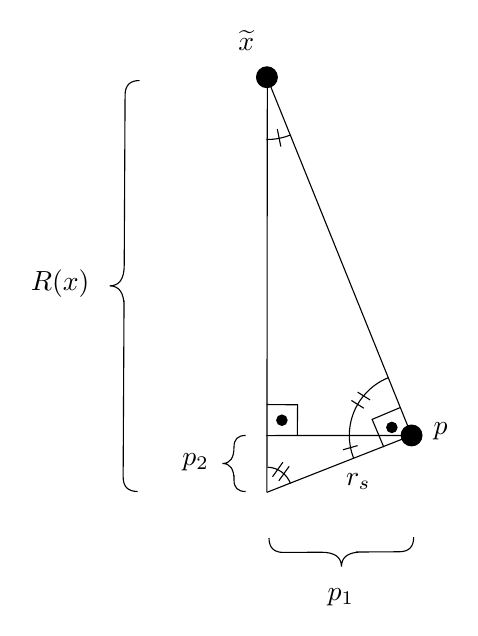
\begin{tikzpicture}[x=0.75pt,y=0.75pt,yscale=-1,xscale=1]
			%uncomment if require: \path (0,306); %set diagram left start at 0, and has height of 306
			
			%Straight Lines [id:da9775960700470973] 
			\draw    (175,225) -- (244.7,197.6) ;
			%Shape: Circle [id:dp650777308898062] 
			\draw  [fill={rgb, 255:red, 0; green, 0; blue, 0 }  ,fill opacity=1 ] (170,25) .. controls (170,22.24) and (172.24,20) .. (175,20) .. controls (177.76,20) and (180,22.24) .. (180,25) .. controls (180,27.76) and (177.76,30) .. (175,30) .. controls (172.24,30) and (170,27.76) .. (170,25) -- cycle ;
			%Straight Lines [id:da5196614062255183] 
			\draw    (244.7,197.6) -- (175,25) ;
			%Straight Lines [id:da023107276049729397] 
			\draw    (175,225) -- (175.2,25) ;
			%Shape: Right Angle [id:dp16259454868629664] 
			\draw   (231.32,203.23) -- (225.69,189.86) -- (239.07,184.22) ;
			%Shape: Circle [id:dp6072225367769397] 
			\draw  [fill={rgb, 255:red, 0; green, 0; blue, 0 }  ,fill opacity=1 ] (232.7,193.73) .. controls (232.7,192.35) and (233.81,191.23) .. (235.2,191.23) .. controls (236.58,191.23) and (237.7,192.35) .. (237.7,193.73) .. controls (237.7,195.11) and (236.58,196.23) .. (235.2,196.23) .. controls (233.81,196.23) and (232.7,195.11) .. (232.7,193.73) -- cycle ;
			%Shape: Circle [id:dp22711373540182844] 
			\draw  [fill={rgb, 255:red, 0; green, 0; blue, 0 }  ,fill opacity=1 ] (239.7,197.6) .. controls (239.7,194.84) and (241.94,192.6) .. (244.7,192.6) .. controls (247.46,192.6) and (249.7,194.84) .. (249.7,197.6) .. controls (249.7,200.36) and (247.46,202.6) .. (244.7,202.6) .. controls (241.94,202.6) and (239.7,200.36) .. (239.7,197.6) -- cycle ;
			%Straight Lines [id:da4664659203823376] 
			\draw    (174.7,197.65) -- (244.7,197.6) ;
			%Shape: Right Angle [id:dp8699104557243595] 
			\draw   (174.83,182.7) -- (189.77,182.83) -- (189.65,197.78) ;
			%Shape: Circle [id:dp7106050260488861] 
			\draw  [fill={rgb, 255:red, 0; green, 0; blue, 0 }  ,fill opacity=1 ] (179.72,190.26) .. controls (179.72,188.88) and (180.83,187.76) .. (182.22,187.76) .. controls (183.6,187.76) and (184.72,188.88) .. (184.72,190.26) .. controls (184.72,191.64) and (183.6,192.76) .. (182.22,192.76) .. controls (180.83,192.76) and (179.72,191.64) .. (179.72,190.26) -- cycle ;
			%Shape: Arc [id:dp039110098125089365] 
			\draw  [draw opacity=0] (186.39,52.84) .. controls (182.93,54.23) and (179.16,55) .. (175.2,55) .. controls (175.04,55) and (174.87,55) .. (174.71,55) -- (175.2,25) -- cycle ; \draw   (186.39,52.84) .. controls (182.93,54.23) and (179.16,55) .. (175.2,55) .. controls (175.04,55) and (174.87,55) .. (174.71,55) ;  
			%Shape: Arc [id:dp4388763820391758] 
			\draw  [draw opacity=0] (216.78,208.59) .. controls (215.44,205.19) and (214.7,201.48) .. (214.7,197.6) .. controls (214.7,185) and (222.47,174.21) .. (233.48,169.77) -- (244.7,197.6) -- cycle ; \draw   (216.78,208.59) .. controls (215.44,205.19) and (214.7,201.48) .. (214.7,197.6) .. controls (214.7,185) and (222.47,174.21) .. (233.48,169.77) ;  
			%Shape: Arc [id:dp13478808103957818] 
			\draw  [draw opacity=0] (175.21,212.89) .. controls (180.31,212.98) and (184.64,216.22) .. (186.34,220.75) -- (175,225) -- cycle ; \draw   (175.21,212.89) .. controls (180.31,212.98) and (184.64,216.22) .. (186.34,220.75) ;  
			%Straight Lines [id:da4590163291530882] 
			\draw    (180,50) -- (181.7,58.4) ;
			%Straight Lines [id:da276145533339089] 
			\draw    (182.7,210.48) -- (177.7,217.48) ;
			%Straight Lines [id:da9764373037016407] 
			\draw    (185.7,212.48) -- (180.7,219.48) ;
			%Straight Lines [id:da32627663759895154] 
			\draw    (218.7,202.48) -- (211.7,204.48) ;
			%Straight Lines [id:da23387251570318401] 
			\draw    (224.7,180.48) -- (218.7,176.73) ;
			%Straight Lines [id:da6122161603078776] 
			\draw    (221.7,184.48) -- (215.7,180.73) ;
			%Shape: Brace [id:dp2795050639782527] 
			\draw   (176,247) .. controls (176.03,251.67) and (178.37,253.99) .. (183.04,253.96) -- (200.89,253.86) .. controls (207.56,253.82) and (210.9,256.13) .. (210.93,260.8) .. controls (210.9,256.13) and (214.22,253.78) .. (220.89,253.74)(217.89,253.76) -- (238.74,253.64) .. controls (243.41,253.61) and (245.73,251.27) .. (245.7,246.6) ;
			%Shape: Brace [id:dp4580887156849429] 
			\draw   (164.7,197.6) .. controls (160.99,197.6) and (159.14,199.45) .. (159.14,203.16) -- (159.14,203.16) .. controls (159.14,208.45) and (157.29,211.1) .. (153.58,211.1) .. controls (157.29,211.1) and (159.14,213.75) .. (159.14,219.04)(159.14,216.66) -- (159.14,219.04) .. controls (159.14,222.75) and (160.99,224.6) .. (164.7,224.6) ;
			%Shape: Brace [id:dp8392881207389759] 
			\draw   (113.7,26.6) .. controls (109.03,26.57) and (106.69,28.89) .. (106.66,33.56) -- (106.25,115.56) .. controls (106.22,122.23) and (103.87,125.55) .. (99.2,125.53) .. controls (103.87,125.55) and (106.18,128.89) .. (106.15,135.56)(106.16,132.56) -- (105.73,217.56) .. controls (105.71,222.23) and (108.03,224.57) .. (112.7,224.6) ;
			
			% Text Node
			\draw (160,1.4) node [anchor=north west][inner sep=0.75pt]    {$\widetilde{x}$};
			% Text Node
			\draw (211.85,214.7) node [anchor=north west][inner sep=0.75pt]    {$r_s$};
			% Text Node
			\draw (254,190) node [anchor=north west][inner sep=0.75pt]    {$p$};
			% Text Node
			\draw (133,205) node [anchor=north west][inner sep=0.75pt]    {$p_2$};
			% Text Node
			\draw (203,270) node [anchor=north west][inner sep=0.75pt]    {$p_1$};
			% Text Node
			\draw (60,116.4) node [anchor=north west][inner sep=0.75pt]    {$R(x)$};
		\end{tikzpicture}
	\end{center}
	We'll use similarity of triangles for the biggest and smallest triangles in the picture. The quotient of the lengths of the sides opposite to the angle with a single stroke and the one opposite to the right angle is the same for each triangle. This implies that
	\begin{equation}
		\frac{p_2}{r_s} = \frac{r_s}{R(x)},
	\end{equation}
	so
	\begin{equation}
		p_2 = \frac{r_s^2}{R(x)}.
	\end{equation}
	The other coordinate $p_1$ is computed using Pythagoras's theorem:
	\begin{equation}
		p_1 = \sqrt{r_s^2-p_2^2} = r_s \ \sqrt{1 - \frac{r_s^2}{R(x)^2}}.
	\end{equation}
	Then
	\begin{equation}
		\label{equation: p}
		p = r_s \left( \sqrt{1 - \frac{r_s^2}{R(x)^2}} \ x^\perp +  \frac{r_s}{R(x)} x \right).
	\end{equation}
	
	Next we find an expression for $q$. It is a convex combination of $\widetilde{x}$ and $p$, so it can be written as
	\begin{equation}
		q = t_1 \widetilde{x} + t_2 p,
	\end{equation}
	where $t_1, t_2 \geq 0$ and $t_1 + t_2 = 1$. The weights $t_1$ and $t_2$ are determined using trigonometry. Writing $q$ with respect to the vectors $x$ and $x^\perp$, we get that
	\begin{align*}
		q &\stackrel{(i)}{=} t_1 R(x) x  + t_2 r_s \left( \sqrt{1 - \frac{r_s^2}{R(x)^2}} \ x^\perp +  \frac{r_s}{R(x)} x \right) \\
		&\stackrel{(ii)}{=} t_2 r_s \sqrt{1 - \frac{r_s^2}{R(x)^2}} \ x^\perp + \left( t_1 R(x) + t_2 \frac{r_s^2}{R(x)} \right) x.
	\end{align*}
	In $(i)$ were used equations \ref{equation: tilde x} and \ref{equation: p}; in $(ii)$ the coefficients of $x^\perp$ and $x$ were grouped together. Since $q$ is a multiple of $\widetilde{x'}$, the quotient of its coordinates must equal the quotient of the coordinates of $\widetilde{x'}$. This is enough to determine the weights $t_i$. We have that
	\begin{equation}
		\frac{t_1 R(x) + t_2 \frac{r_s^2}{R(x)} }{ t_2 r_s \sqrt{1 - \frac{r_s^2}{R(x)^2}} } = \frac{|\widetilde{x'}_2|}{|\widetilde{x'}_1|}.
	\end{equation}
	We can pass the $t_2$ in the denominator to the nominator, dividing it:
	\begin{equation}
		\frac{\frac{t_1}{t_2} R(x) + \frac{r_s^2}{R(x)} }{ r_s \sqrt{1 - \frac{r_s^2}{R(x)^2}} } = \frac{|\widetilde{x'}_2|}{|\widetilde{x'}_1|}.
	\end{equation}
	Isolating $t_1 / t_2$, we get that
	\begin{equation}
		\label{equation: weights quotient 1}
		\frac{t_1}{t_2} = \frac{|\widetilde{x'}_2|}{|\widetilde{x'}_1|} \frac{r_s}{R(x)} \sqrt{1 - \frac{r_s^2}{R(x)^2}} -\frac{r_s^2}{R(x)^2}.
	\end{equation}
	Let's give a name to the right side. Define the function
	\begin{equation}
		\label{equation: f}
		f(x, x') \coloneqq \frac{|\widetilde{x'}_2|}{|\widetilde{x'}_1|} \frac{r_s}{R(x)} \sqrt{1 - \frac{r_s^2}{R(x)^2}} -\frac{r_s^2}{R(x)^2} .
	\end{equation}
	Equation \ref{equation: weights quotient 1} then becomes
	\begin{equation}
		\frac{t_1}{t_2} = f(x, x').
	\end{equation}
	Isolating $t_1$, we get that
	\begin{equation}
		\label{equation: weights quotient 2}
		t_1 = f(x, x') t_2.
	\end{equation}
	The weights also sum to 1, so
	\begin{equation}
		\label{equation: t2 = 1-t1}
		t_2 = 1-t_1.
	\end{equation}
	Substituting this expression in equation \ref{equation: weights quotient 2}, we get that
	\begin{equation}
		t_1 = f(x, x') (1-t_1) = f(x, x') - f(x, x') t_1.
	\end{equation}
	Isolating $t_1$, we get that
	\begin{equation}
		\label{equation: t1}
		t_1 = \frac{f(x, x')}{1 + f(x, x')}.
	\end{equation}
	We obtain $t_2$ from equation \ref{equation: t2 = 1-t1}:
	\begin{align*}
		t_2 &\stackrel{(i)}{=} 1-t_1 \\
		&\stackrel{(ii)}{=} 1 -\frac{f(x, x')}{1 + f(x, x')} \\
		&\stackrel{(iii)}{=} \frac{1+f(x, x') - f(x, x')}{1 + f(x, x')} \\
		&\stackrel{(iv)}{=} \frac{1}{1+f(x, x')}.
	\end{align*}
	In $(i)$ was used equation \ref{equation: t2 = 1-t1}; in $(ii)$ was used equation \ref{equation: t1}; in $(iii)$ the subtraction of numbers was turned into a single fraction; in $(iv)$ the $f(x')$ in the nominator was canceled. This proves that
	\begin{equation}
		\label{equation: t2}
		t_2 = \frac{1}{1+f(x, x')}.
	\end{equation}
	Previously we proved that
	\begin{equation}
		\label{equation: q}
		q = t_2 r_s \sqrt{1 - \frac{r_s^2}{R(x)^2}} \ x^\perp + \left( t_1 R(x) + t_2 \frac{r_s^2}{R(x)} \right) x.
	\end{equation}
	Having determined the weights $t_i$, we finished determining $q$.
	
	We'll use $q$ to estimate $R(x')$, since $R(x') \geq ||q||$. We'll see later that $\lim_{x' \to x} t_1 = 1$ and $\lim_{x' \to x} t_2 = 0$, so the relevant term of $q$ is $t_1 R(x)$. We can estimate $||q||$ as follows. From Pythagoras's theorem, we have that
	\begin{equation}
		||q||^2 = \left( t_2 r_s \sqrt{1 - \frac{r_s^2}{R(x)^2}} \ \right)^2 + \left( t_1 R(x) + t_2 \frac{r_s^2}{R(x)} \right)^2.
	\end{equation}
	Dropping the first square in the sum of squares and using that every term is non negative, we get that
	\begin{equation}
		||q|| \geq t_1 R(x) + t_2 \frac{r_s^2}{R(x)}.
	\end{equation}
	The term that contains $t_2$ is non negative, dropping it we get that
	\begin{equation}
		||q|| \geq t_1 R(x).
	\end{equation}
	Since $R(x') \geq ||q||$, this implies that
	\begin{equation}
		R(x') \geq t_1 R(x).
	\end{equation}
	Let's make the dependence on $x$ and $x'$ explicit. Using equation \ref{equation: t1}, we get that
	\begin{equation}
		R(x') \geq \frac{f(x,x')}{1+f(x,x')} R(x).
	\end{equation}
	Swapping $x$ and $x'$, we also have that
	\begin{equation}
		R(x) \geq \frac{f(x',x)}{1+f(x',x)} R(x').
	\end{equation}
	Isolating $R(x')$, we get that
	\begin{equation}
		\frac{1+f(x',x)}{f(x',x)} R(x) \geq R(x').
	\end{equation}
	The inequalities together imply that
	\begin{equation}
		\label{equation: R(x') bounds}
		\frac{f(x,x')}{1+f(x,x')} R(x) \leq R(x') \leq \frac{1+f(x',x)}{f(x',x)} R(x).
	\end{equation}
	To prove that $\lim_{x' \to x} R(x') = R(x)$, we'll show that:
	\begin{equation}
		\lim_{x' \to x} \frac{f(x,x')}{1+f(x,x')} = 1,
	\end{equation}
	\begin{equation}
		\lim_{x' \to x} \frac{1+f(x',x)}{f(x',x)} = 1.
	\end{equation}
	
	Before computing these limits, let's find a coordinate free expression for $f(x,x')$. The function was defined as
	\begin{equation}
		f(x, x') = \frac{|\widetilde{x'}_2|}{|\widetilde{x'}_1|} \frac{r_s}{R(x)} \sqrt{1 - \frac{r_s^2}{R(x)^2}} -\frac{r_s^2}{R(x)^2} .
	\end{equation}
	The relevant part is the fraction $|\widetilde{x'}_2| / |\widetilde{x'}_1|$. The components are related to $||\widetilde{x'}||$ by Pythagoras's theorem:
	\begin{equation}
		\label{equation: ||x' tilde|| pythagoras}
		||\widetilde{x'}||^2 = |\widetilde{x'}_1|^2 + |\widetilde{x'}_2|^2 .
	\end{equation}
	Using that $||\widetilde{x'}|| = R(x')$, we have that
	\begin{equation}
		\label{equation: x' tilde 1}
		|\widetilde{x'}_1| = \sqrt{R(x')^2 - |\widetilde{x'}_2|^2 }.
	\end{equation}
	From equation \ref{equation: x' in base}, the coordinate $\widetilde{x'}_2$ is given by the inner product
	\begin{equation}
		\widetilde{x'}_2 = \widetilde{x'} \cdot x.
	\end{equation}
	Taking the absolute value and using that $\widetilde{x'} = R(x') x'$, we get that:
	\begin{equation}
		|\widetilde{x'}_2 | = R(x') \ x' \cdot x.
	\end{equation}
	Again, by equation \ref{equation: x x' > 0}, we are assuming that $x \cdot x' > 0$. Substituting in equation \ref{equation: x' tilde 1}, we get that
	\begin{align*}
		|\widetilde{x'}_1| &= \sqrt{R(x')^2 - R(x')^2 (x' \cdot x )^2 } \\
		&= R(x') \sqrt{1 - (x' \cdot x )^2 }.
	\end{align*}
	In the last equality, the term $R(x')$ was factored. Next we use this result to find an expression for $|\widetilde{x'}_2|/|\widetilde{x'}_1|$. Using again equation \ref{equation: ||x' tilde|| pythagoras} and that $||\widetilde{x'}|| = R(x')$, we have that
	\begin{equation}
		\label{equation: x'tilde 2}
		|\widetilde{x'}_2| = \sqrt{R(x')^2 - |\widetilde{x'}_1|^2 }.
	\end{equation}
	Dividing by $|\widetilde{x'}_1 |$, we get that
	\begin{align*}
		\frac{|\widetilde{x'}_2|}{|\widetilde{x'}_1|} &\stackrel{(i)}{=} \sqrt{\frac{R(x')^2}{|\widetilde{x'}_1|^2} - 1 } \\
		&\stackrel{(ii)}{=} \sqrt{ \frac{1}{1 - (x' \cdot x )^2} -1}.
	\end{align*}
	In $(i)$ was used equation \ref{equation: x'tilde 2}; in $(ii)$ was used the expression for $|\widetilde{x'}_1|$. Substituting the expression for $|\widetilde{x'}_2| / |\widetilde{x'}_1|$ into the definition of $f$, as in equation \ref{equation: f}, we get that
	\begin{equation}
		\label{equation: f coordinate free}
		f(x,x') = \sqrt{ \frac{1}{1 - (x' \cdot x)^2} -1} \ \frac{r_s}{R(x)} \sqrt{1 - \frac{r_s^2}{R(x)^2}} -\frac{r_s^2}{R(x)^2}
	\end{equation}
	
	Next, let's compute $\lim_{x' \to x} f(x,x')$. As $x'$ approaches $x$, $x' \cdot x$ approaches $1$ from below. Therefore, $1 - (x' \cdot x)^2$ approaches $0$ from above as $x'$ approaches $x$. Then
	\begin{equation}
		\label{equation: limit square root}
		\lim_{x' \to x} \sqrt{ \frac{1}{1 - (x' \cdot x )^2} -1} = +\infty .
	\end{equation}
	Since
	\begin{equation}
		\frac{r_s}{R(x)} \sqrt{1 - \frac{r_s^2}{R(x)^2}} > 0,
	\end{equation}
	it follows that
	\begin{equation}
		\lim_{x' \to x} \sqrt{ \frac{1}{1 - (x' \cdot x )^2} -1} \ \frac{r_s}{R(x)} \sqrt{1 - \frac{r_s^2}{R(x)^2}} = +\infty.
	\end{equation}
	The remaining term of $f(x, x')$ doesn't depend on $x'$, so
	\begin{equation}
		\lim_{x' \to x} f(x, x') = +\infty.
	\end{equation}
	Then
	\begin{align*}
		\lim_{x' \to x} \frac{f(x,x')}{1+f(x,x')} &\stackrel{(i)}{=} \lim_{x' \to x} \frac{1+f(x,x')-1}{1+f(x,x')} \\
		&\stackrel{(ii)}{=} 1-\lim_{x' \to x} \frac{1}{1+f(x,x')} \\
		&\stackrel{(iii)}{=} 1 - 0 \\
		&= 1.
	\end{align*}
	In $(i)$ was added and subtracted 1 from the numerator; in $(ii)$ the term $1+f(x,x')$ from the numerator was divided by the denominator, obtaining 1; in $(iii)$ was used that $\lim_{x' \to x} f(x, x') = +\infty$. This proves that
	\begin{equation}
		\label{equation: limit fraction left}
		\lim_{x' \to x} \frac{f(x,x')}{1+f(x,x')} = 1.
	\end{equation}
	As said earlier, we would compute $\lim_{x' \to x} t_1$, which is the limit just computed. Since $t_2 = 1 - t_1$, of course $\lim_{x' \to x} t_2 = 0$.
	
	Now let's compute $\lim_{x' \to x} f(x', x)$. Swapping $x$ and $x'$ in equation \ref{equation: f coordinate free}, we get that
	\begin{equation}
		f(x', x) = \sqrt{ \frac{1}{1 - (x \cdot x' )^2} -1} \ \frac{r_s}{R(x')} \sqrt{1 - \frac{r_s^2}{R(x')^2}} -\frac{r_s^2}{R(x')^2}.
	\end{equation}
	The first square root is invariant by the swap, so we already know its limit, which is $+\infty$, as shown in equation \ref{equation: limit square root}. This time the other terms depend on $x'$, which makes it harder to compute the limit. By equation \ref{equation: R bounds}, $R(x')$ is bounded by $r_{min} \leq R(x') \leq r_{max}$. It follows that
	\begin{equation}
		\label{equation: bound 1}
		\frac{r_s}{R(x')} \sqrt{1 - \frac{r_s^2}{R(x')^2}} \geq \frac{r_s}{r_{max}} \sqrt{1 - \frac{r_s^2}{r_{min}^2}},
	\end{equation}
	\begin{equation}
		\label{equation: bound 2}
		-\frac{r_s^2}{R(x')^2} \geq -\frac{r_s^2}{r_{min}^2}.
	\end{equation}
	Notice that if we used $r_{min}$ instead of $r_s$, we would get the bound
	\begin{equation}
		\frac{r_{min}}{R(x')} \sqrt{1 - \frac{r_{min}^2}{R(x')^2}} \geq \frac{r_{min}}{r_{max}} \sqrt{1 - \frac{r_{min}^2}{r_{min}^2}} = 0,
	\end{equation}
	which is useless for computing the limit. Using the limit from equation \ref{equation: limit square root} and the bounds from equations \ref{equation: bound 1} and \ref{equation: bound 2}, it follows that
	\begin{equation}
		\lim_{x' \to x} f(x', x) = +\infty.
	\end{equation}
	Then
	\begin{align*}
		\lim_{x' \to x} \frac{1+f(x',x)}{f(x',x)} &\stackrel{(i)}{=} \frac{1}{f(x', x)} +1\\
		&\stackrel{(ii)}{=} 0+1 \\
		&= 1.
	\end{align*}
	In $(i)$ the $f(x', x)$ from the numerator was divided by the denominator, obtaining 1; in $(ii)$ was used that $\lim_{x' \to x} f(x', x) = +\infty$. This proves that
	\begin{equation}
		\label{equation: limit fraction right}
		\lim_{x' \to x} \frac{1+f(x',x)}{f(x',x)} = 1.
	\end{equation}
	
	The inequalities from equation \ref{equation: R(x') bounds} together with the limits from equations \ref{equation: limit fraction left} and \ref{equation: limit fraction right} imply that
	\begin{equation}
		\lim_{x' \to x} R(x') = R(x).
	\end{equation}
	This concludes that $R$ is a continuous function.
	
	It is immediate that $\varphi$ is continuous over $C' \setminus \{0\}$, because it is constructed from continuous functions. To prove that $\varphi$ is continuous, it remains to show the continuity at 0, that is,
	\begin{equation}
		\lim_{x \to 0} \varphi(x) = 0.
	\end{equation}
	We can assume when computing the limit that $x \neq 0$, so
	\begin{equation}
		\varphi(x) = \frac{x}{R(x/||x||)}.
	\end{equation}
	Taking the norm, we have that
	\begin{equation}
		||\varphi(x)|| = \frac{||x||}{R(x/||x||)}.
	\end{equation}
	By equation \ref{equation: R bounds}, we have that $R(x/||x||) \geq r_{min}$, so
	\begin{equation}
		||\varphi(x)|| \leq \frac{||x||}{r_{min}}.
	\end{equation}
	It follows from this inequality that
	\begin{equation}
		\lim_{x \to 0} \varphi(x) = 0.
	\end{equation}
	This concludes that $\varphi$ is a continuous function. The inverse is given by
	\begin{equation}
		\varphi^{-1}(x) = \begin{cases}
			R\left(\frac{x}{||x||}\right) x, &\text{ if } x \in \overline{B(0,1)} \setminus \{0\}, \\
			0, &\text{ if } x = 0.
		\end{cases}
	\end{equation}
	It continuous over $\overline{B(0,1)} \setminus \{0\}$, because it is constructed from continuous functions. From equation \ref{equation: R bounds}, we know that $R(x/||x||) \leq r_{max}$, so
	\begin{equation}
		||\varphi^{-1}(x)|| \leq r_{max} ||x||,
	\end{equation}
	for $x \in \overline{B(0,1)} \setminus \{0\}$. It follows that
	\begin{equation}
		\lim_{x \to 0} \varphi^{-1} (x) = 0.
	\end{equation}
	Therefore, $\varphi^{-1}$ is a continuous function, so $\varphi$ is a homeomorphism.
\end{proof}

\end{document}
